\section{Evaluation}  \label{sec:evaluation} 
The proposed obstacle aware controller\footnote{Source code: \url{https://github.com/hubernikus/obstacle_aware_damping}} is compared to a baseline, the velocity preserving, passive controller \parencite{kronander2015passive}.

\subsection{Qualitative Comparison} \label{sec:qual_comp}
A qualitative analysis of the proposed controller's behavior in three scenarios, as depicted in Figure~\ref{fig:obstacle_aware_damping_comparison}. In each scenario, the agent approaches multiple obstacles from distinct starting positions, a disturbance (indicated by an arrow) is applied. The simulation time step is $\Delta t = 0.01 s$ seconds, and the agent's mass matrix is $\matd{M} = \matr{I} kg$. The controller is implemented using the following damping values:
$s^{\mathrm{obs}}=~$\qty{200}{s^{-1}},
$s^{\mathrm{f}}=$~\qty{100}{s^{-1}}, and
$s^{\mathrm{c}}=$~\qty{20}{s^{-1}}.

In the top trajectory, the robot encounters a stand-alone obstacle and experiences a disturbance that pushes it toward the obstacle. With the obstacle-aware controller, the robot avoids collision and continues moving towards the attractor. In contrast, the baseline controller, which prioritizes velocity conservation, fails to respond effectively and is pushed into the obstacle, resulting in a colliding trajectory.

During the middle trajectory, a disturbance occurs when the agent is positioned between two obstacles. The obstacle-aware controller utilizes the normal vector $\vect n(\vecs \xi)$, as described in Section~\ref{sec:obstacle_repulsion}. However, due to its construction, the magnitude of $\vect n(\vecs \xi)$ diminishes in narrow passages (as seen in \eqref{eq:averaged_normal}), leading to increased damping in all directions, as described in \eqref{eq:leaving_compliance}. As a result, the agent successfully avoids the disturbance using the obstacle-aware controller, while the baseline controller follows a colliding trajectory.

In the bottom trajectory, the repulsive force points away from the obstacle. The obstacle-aware and the velocity-preserving controllers produce nearly identical trajectories due to equal compliance when moving away from an obstacle as defined in \eqref{eq:leaving_compliance}.

We observe the selective damping of disturbances towards the obstacle. The top and middle disturbances are highly damped, while the bottom disturbances are not. This feature imparts a natural behavior of moving away from obstacles.
% Furthermore, in Fig.~\ref{fig_run_damped_towards}, one can observe the feature described in Section~\ref{sec:damping_only_toward}, that only damps the disturbance towards the obstacle. The first disturbance is highly damped, while the second is much less. This feature provides a natural behavior of moving away from obstacles, improving the margin of impenetrability. 

\begin{figure}[htbp]
  \centering
  \centerline{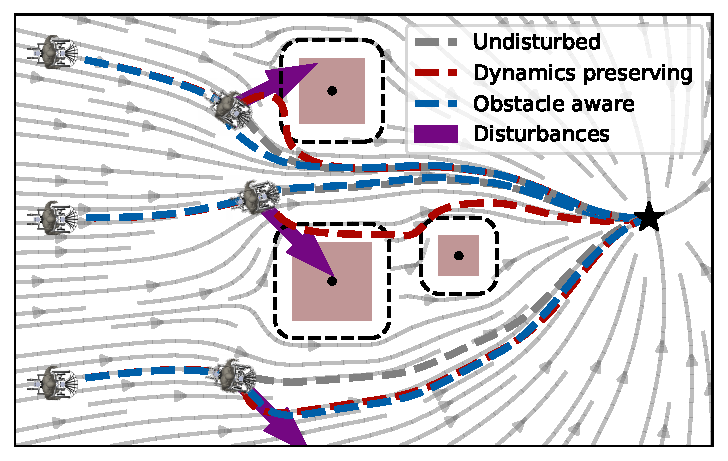
\includegraphics[width=0.95\columnwidth]{figures/multi_obstacle_with_damping.pdf}}
  \caption{
  The desired velocity $\vect f(\vecs \xi)$ is represented in gray and serves as the input for the force controller. The mobile robot, initially positioned at three different locations, navigates safely towards the attractor (black star) even when confronted with external disturbances (purple arrows) while employing the obstacle-aware controller (blue trajectories). In contrast, the baseline controller (red) results in collisions when disturbances occur close to the robot.
  }
  \label{fig:obstacle_aware_damping_comparison}
\end{figure}

\subsection{Noise Analysis}
In practical robotic applications, controllers are inevitably exposed to noise and unexpected disturbances, arising from sensor inaccuracies, environmental factors, or other external perturbations. A high-quality controller can effectively reject such disturbances while simultaneously achieving the control objectives, such as collision avoidance and trajectory tracking.

This section investigates the impact of noise disturbances on a simulated agent with an identity mass matrix $\matd M = \matr I kg$. The discrete time step is set to $\Delta t = $~\qty{0.2}{s}. Additionally, the damping values are configured as follows: 
$s^{\mathrm{obs}}=$~\qty{50}{s^{-1}},
$s^{\mathrm{f}}=$~\qty{40}{s^{-1]}}, and
$s^{\mathrm{c}}=$~\qty{5}{s^{-1}}.
The robot's objective is to follow a linear velocity field of the form $\vect f(\vecs \xi) = (\vecs \xi^a - \vecs \xi)$ with a velocity cap of \qty{1}{m/s}.
To evaluate the controller's performance, a comparative analysis is conducted by assessing the minimal distance to the surface along the trajectory, denoted as $ \min_t \| \vecs \xi_t - \vecs \xi^b \| $, with the boundary point $\vecs \xi_b$ described in \eqref{eq:distance_function}. 

\subsubsection{Velocity Noise Resistance}
We first added a normally distributed noise with a zero mean to the agent's velocity $\dot{\vecs{ \xi}}$ at each time step before computing the control force. The agent has to navigate between two obstacles from the starting position to the attractor with different noise levels, as visualized in Figure~\ref{fig:velocity_noise})

The obstacle-aware controller effectively rejects the noise impacting the velocity, even as the noise variance increases. However, the closest distance during the trajectory diminishes with higher noise variance. On the contrary, the velocity-following controller's mean distance falls below zero already at a velocity noise variance of $\qty{0.5}{m/s}$, indicating that many trajectories collide with at least one obstacle.

Furthermore, the obstacle-aware controller maintains a higher minimal distance along the trajectory without noise. This effect results from the higher damping applied towards the obstacle, enabling more precise tracking of the curvature guiding the velocity around the obstacle.

\begin{figure}[htbp]
    \centering
    \begin{subfigure}{\columnwidth}
      \centerline{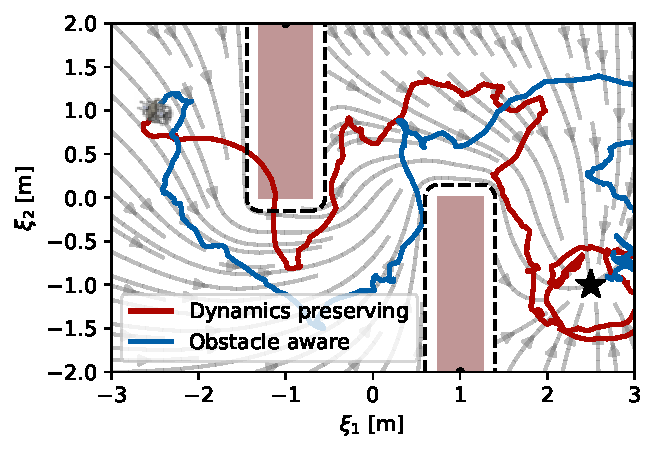
\includegraphics[width=\textwidth]{figures/trajectory_velocity_noise}}
      \caption{Trajectories with a standard deviation of the velocity-noise of 1.0 m/s.}
      \label{fig:trajectory_velocity_noise}
    \end{subfigure}
    \begin{subfigure}{\columnwidth}
    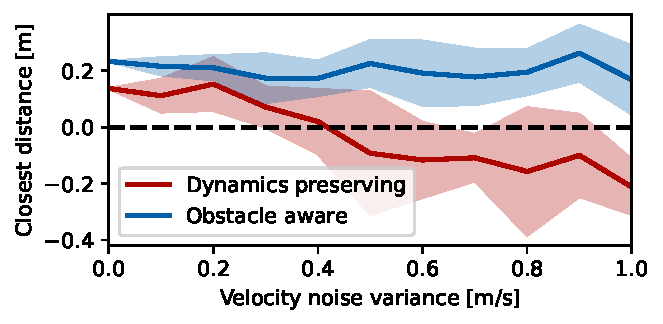
\includegraphics[width=\textwidth]{figures/comparison_velocity_noise}
      \caption{The mean and variance (shaded) of the closest distances over 10 epochs.}
      \label{fig:comparison_velocity_noise}
    \end{subfigure}
	\caption{The agent navigates between two elongated obstacles (a) towards the attractor (black star). The agent's velocity is subjected to white noise, with a mean of zero, and noise variances between \qty{0.0}{m/s} and \qty{1.0}{m/s}. The robot initiates its trajectory from the starting position $\vecs \xi_0 = [-2.5, 1.0]^T$, with an initial velocity of zero. It aims to reach the attractor located at $\vecs \xi^a = [2.5, \, -1.0]^T$.}
\label{fig:velocity_noise}
\end{figure}

\subsubsection{Position Noise Resistance} \label{sec:position_noise}
In the second experiment, normally distributed noise with a mean of zero is added to the position $\vecs{ \xi}$ (Fig.~\ref{fig:position_noise}). The agent has to navigate around two star-shaped obstacles to reach the attractor with various noise levels being applied.

The obstacle-aware controller maintains a greater distance to the surface even when no noise is present, while the velocity-preserving controller already exhibits collisions. As a result, the obstacle-aware creates trajectories with the mean of the distance above zero for standard deviations of the position noise smaller than \qty{0.023}{m}. Conversely, the velocity-preserving controller's mean distance to the surface is below zero for all experiment runs, indicating collisions.
This difference is attributed to the buffer mechanism inherent in the obstacle-aware controller. Despite a similar decrease in distance for both controllers, the obstacle-aware controller effectively prevents collisions due to its higher damping of velocities toward the obstacles.

Moreover, the velocity-preserving controller exhibits a higher distance variance, likely stemming from its lower damping, causing it to adapt more slowly to new velocities after being displaced by the noise. Consequently, this behavior leads to more random variations in velocity and trajectory.

\begin{figure}[htbp]
    \centering
    \begin{subfigure}{\columnwidth}
      \centerline{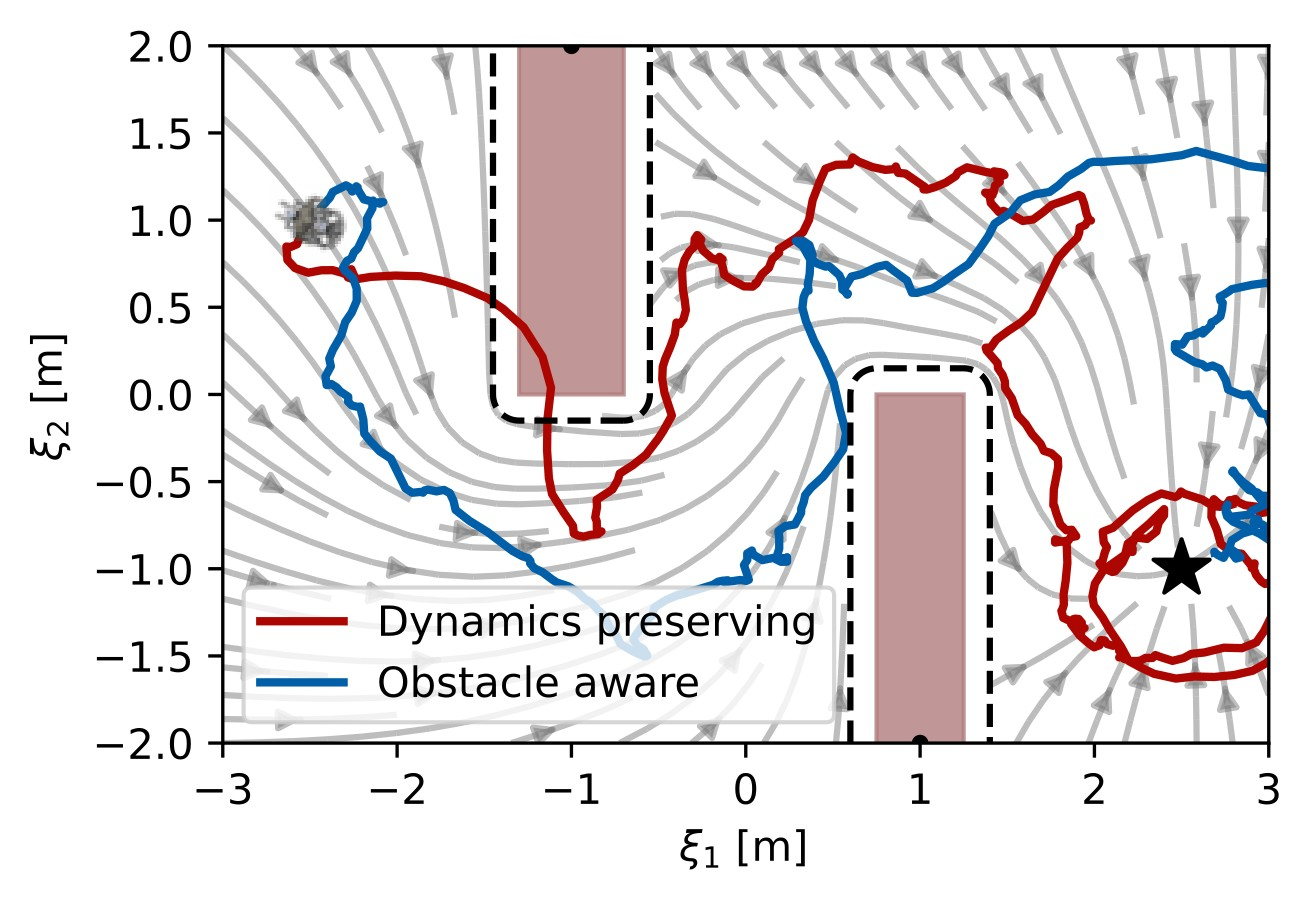
\includegraphics[width=\textwidth]{figures/trajectory_position_noise}}
      \caption{Trajectories with a standard deviation of the position-noise of 0.0 m.}
      \label{fig:trajectory_position_noise}
    \end{subfigure}
    \begin{subfigure}{\columnwidth}
    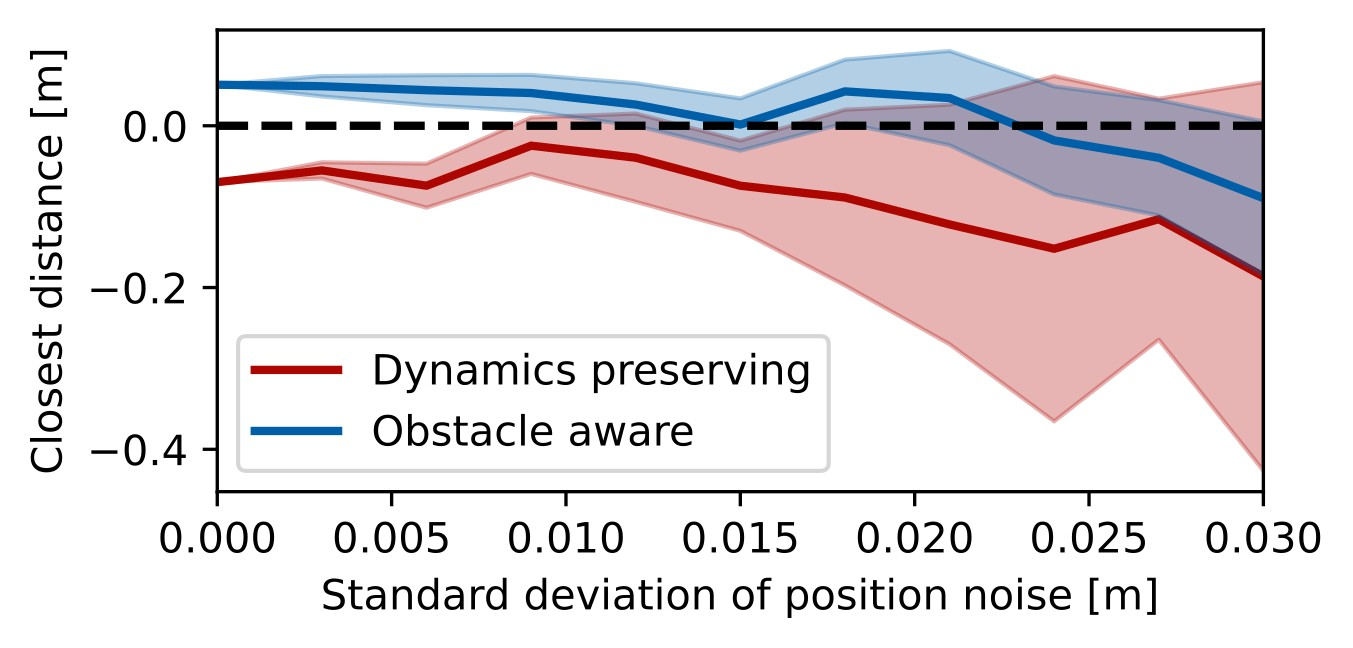
\includegraphics[width=\textwidth]{figures/comparison_position_noise}
      \caption{Closest distances concerning different noise levels over ten epochs.}
      \label{fig:comparison_position_noise}
    \end{subfigure}
	\caption{
 The agent is navigating towards the attractor (black star) between two concave obstacles (a) while being subjected to white noise in its position. The position noise has a mean of zero, and various noise variances ranging between \qty{0.0}{m} and \qty{0.03}{m}. The robot starts at position $\vecs \xi_0 = [-2.5, -1.0]^T$, and the attractor is set to $\vecs \xi^a = [2.5, 1.0]^T$.
 }
\label{fig:position_noise}
\end{figure}


\subsection{Obstacle Aware Passivity Using a Robot Arm}
The obstacle-aware passivity controller was implemented to guide a 7-degree-of-freedom robot arm (Panda from Franka Emika) while moving around a cubic obstacle. 

The joint torque is computed using inverse kinematics combined with the proposed passive controller for the position, but a proportional controller for the orientation:
\begin{equation}
	\vecs \tau_q = \matr J^{\dag}(\vect q) 
	\begin{bmatrix} \matd D(\vecs \xi) \left( \vect f(\vecs \xi) - \dot{\vecs \xi} \right) \\  p^\alpha (\vecs \alpha - \vecs \alpha^a) \end{bmatrix}
\end{equation}
where $\matr J^{\dag}$ represents the Moore-Penrose pseudo inverse of the Jacobian matrix, and $\vecs \alpha$ and $\vecs \alpha^a$ denote the end effector's orientation and the desired orientation, respectively. The angular damping parameter is chosen as $p^\alpha = 5.5$.
The desired orientation $\vecs \alpha^a$ is pointing downward with a quaternion value of $(w, x, y, z) = (0, 1, 0, 0)$. For the angle subtraction, we use quaternion representation to avoid singularities, but an angle-axis representation of the orientation is used to evaluate the torque from the angular offset.

The angular damping is chosen as $p^\alpha = 5.5$.
The damping values are set as
$s^{\mathrm{obs}}=$~\qty{160}{s^{-1}},
$s^{\mathrm{f}}=$~\qty{64}{s^{-1]}}, and
$s^{\mathrm{c}}=$~\qty{16}{s^{-1}}.

The robot start position is approximately at $\vecs \xi_0 = [0.3\mathrm{m}, 0.4\mathrm{m}, 0.3\mathrm{m},]^T$ and the attractor is at position $\vecs \xi^a = [0.26 \mathrm{m}, -0.53\mathrm{m}, 0.33\mathrm{m}]^T$.
The robot encounters a single squared box with axes length \qty{0.16}{m} and a margin of \qty{0.12}{m}, placed in front of the robot base (Fig.~\ref{fig:evaluation_on_robot_arm}). The precise location of the box is tracked in real-time using a marker-based vision system (Optitrack). As the robot passes by the box, it is disturbed by a strong push $\vecs t^e$ towards the box. The experiment is repeated ten times for both controllers, as well as for the undisturbed motion.

The experimental results in \ifthesis Figure~\ref{fig:instances_evaluation_on_robot_arm} and \fi Figure~\ref{fig:evaluation_on_robot_arm} demonstrate that the obstacle-aware controller allows the robot to maintain an average distance of \qty{0.15}{m} away from the obstacle surface. In contrast, the velocity-preserving controller results in a mean distance below \qty{0.05}{m}, and numerous trajectories lead to collisions with the box. On average, the robot passes further away from the obstacle using the obstacle-aware controller and exhibits higher forces, Table~\ref{tab:evaluation_on_robot_arm}.

\begin{table}[htb]
% Distance [NoDist]: 0.1672703839  \pm 0.009033828534378131
% Distance [PassiveDS]: 0.018012260429208955  \pm 0.02613021511175264
% Distance [Aware]: 0.10564614093567434  \pm 0.02136799916777507
% No-Interaction Force: 2.8572200673080523 \pm 0.36821047478539665 
% No-Damping Force: 3.5782840941712544 \pm 0.23762587158014598 
% Obstacle-Aware Force: 4.1208857008362125 \pm 0.25191997294727264 
    \centering
    \begin{tabular}{|l|c|c|c|} \hline
        & Obstacle & Velocity & Undisturbed \\ \hline
         Closest Distance [mm] &  105 $\pm$ 21 & 18 $\pm$ 21 & 167 $\pm$ 9 \\ \hline
         Maximum Force [N] & 4.12 $\pm$ 0.25 & 3.58 $\pm$ 0.24 & 2.86 $\pm$ 0.37  \\ \hline 
    \end{tabular}
    \caption{The mean and standard deviation of the closest distance and maximum force over the ten epochs.}
    \label{tab:evaluation_on_robot_arm}
\end{table}

This outcome is attributed to the obstacle-aware controller's stronger control force, with a high peak occurring around \qty{1.45}{s} when the disturbance is encountered. In contrast, the velocity-preserving controller only reacts when the robot is almost colliding, leading to a delayed response. Additionally, the obstacle-aware controller exhibits higher forces even before the disturbance, which contributes to improved tracking of the avoidance trajectory, as observed in Section~\ref{sec:position_noise}. These findings affirm the superior collision avoidance capabilities and tracking performance of the obstacle-aware passivity controller in real-world robot arm scenarios.

\ifthesis
\begin{figure}[htbp]
    \centering
   \begin{subfigure}{\columnwidth}
    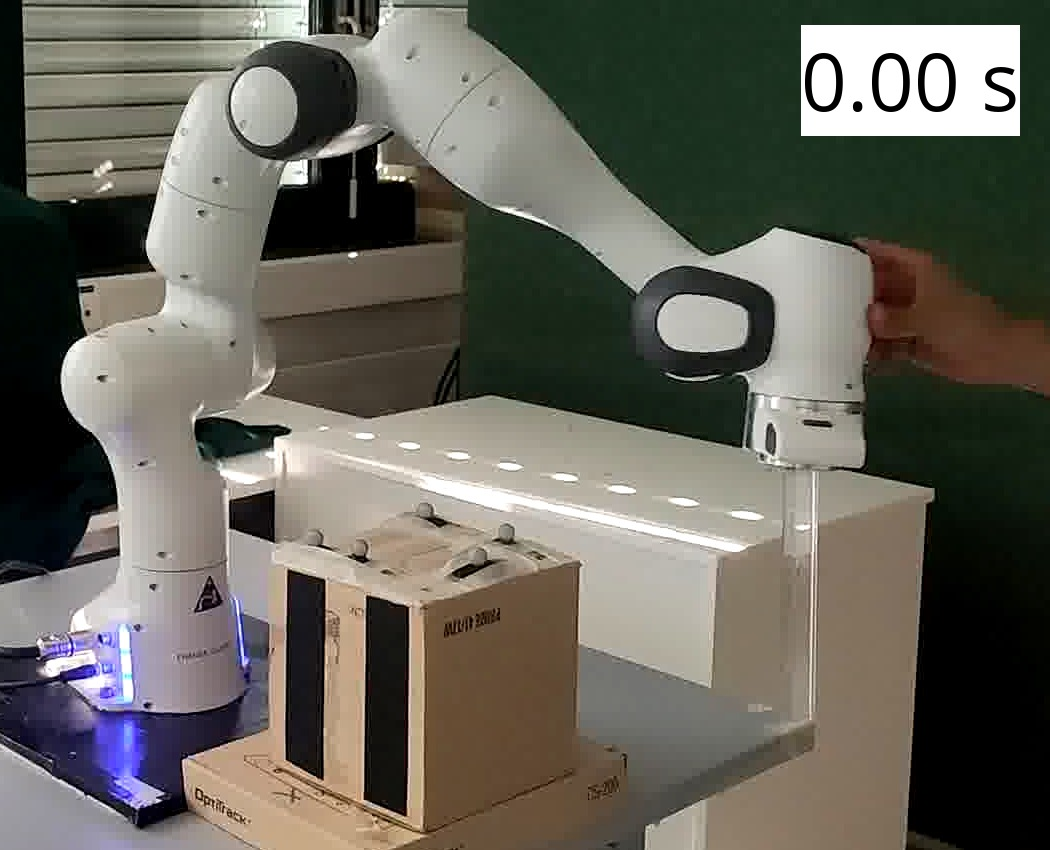
\includegraphics[width=0.4\textwidth]{figures/franka_sequence/franka_obstacle_aware016}\hfill%
    % 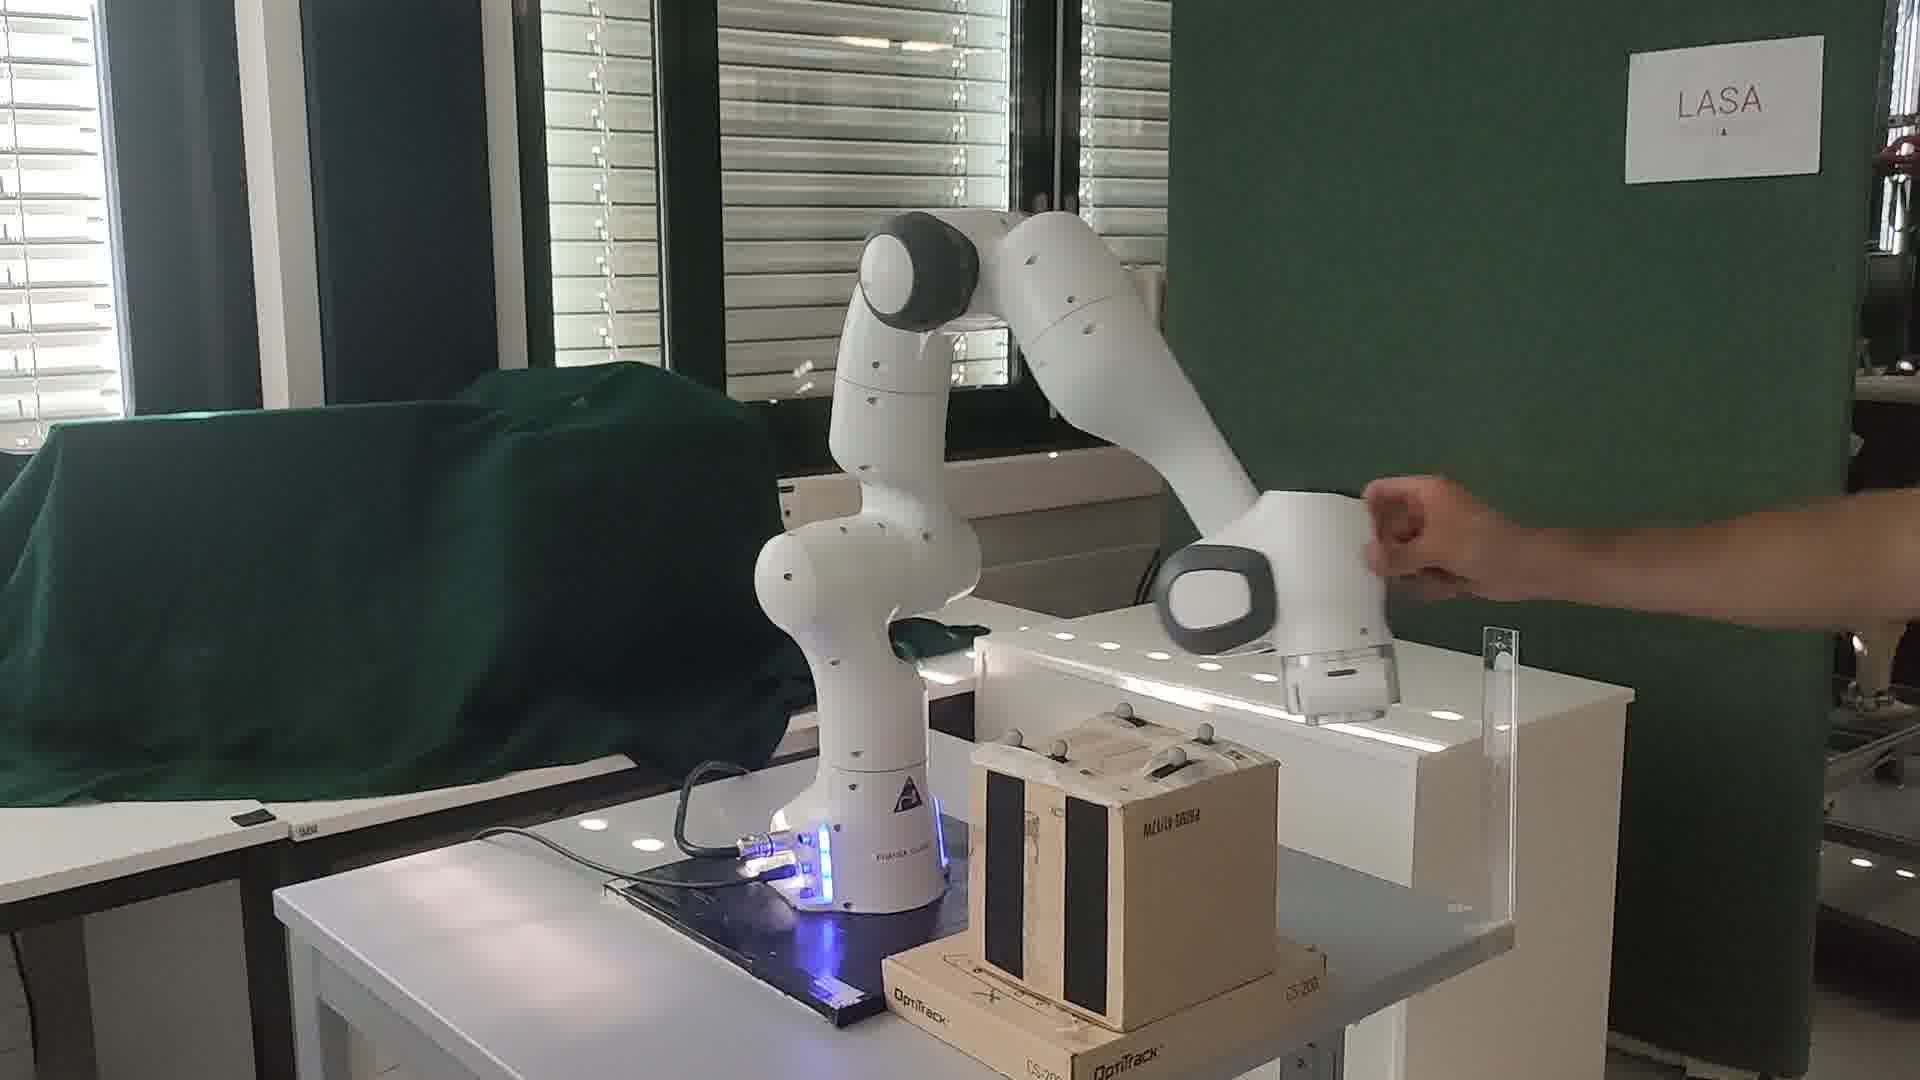
\includegraphics[width=0.33\textwidth]{figures/franka_sequence/franka_obstacle_aware018}\hfill%
    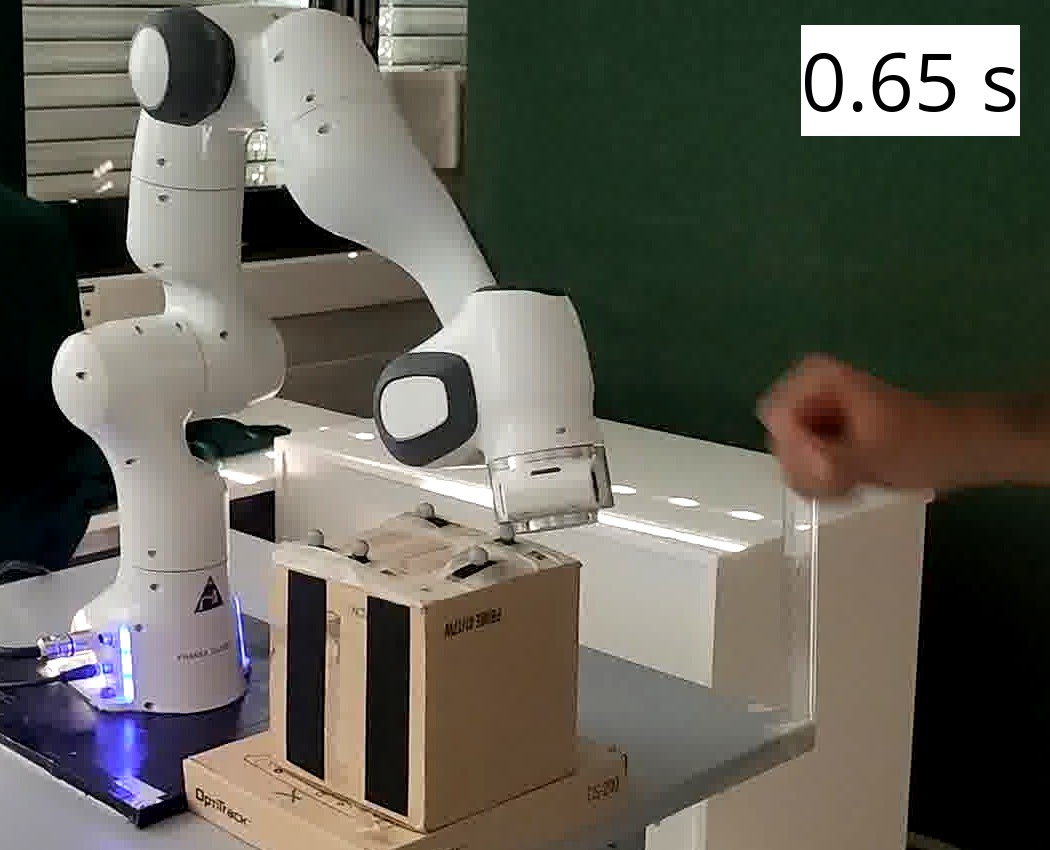
\includegraphics[width=0.4\textwidth]{figures/franka_sequence/franka_obstacle_aware020}
      \caption{Obstacle-aware controller rejects repulsion and avoids collision}
      \label{fig:franka_sequence_obstacle_aware}
    \end{subfigure}
	\begin{subfigure}{\columnwidth}
    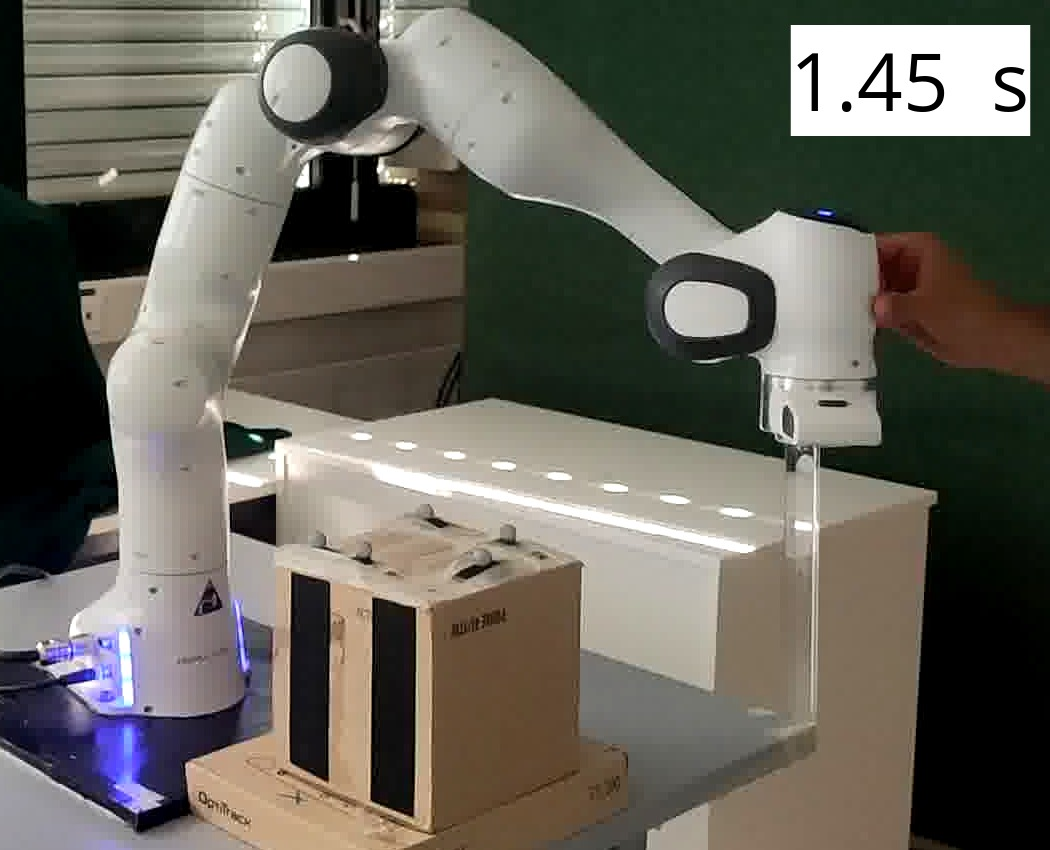
\includegraphics[width=0.4\textwidth]{figures/franka_sequence/franka_velocity_conserving021}\hfill%
    % 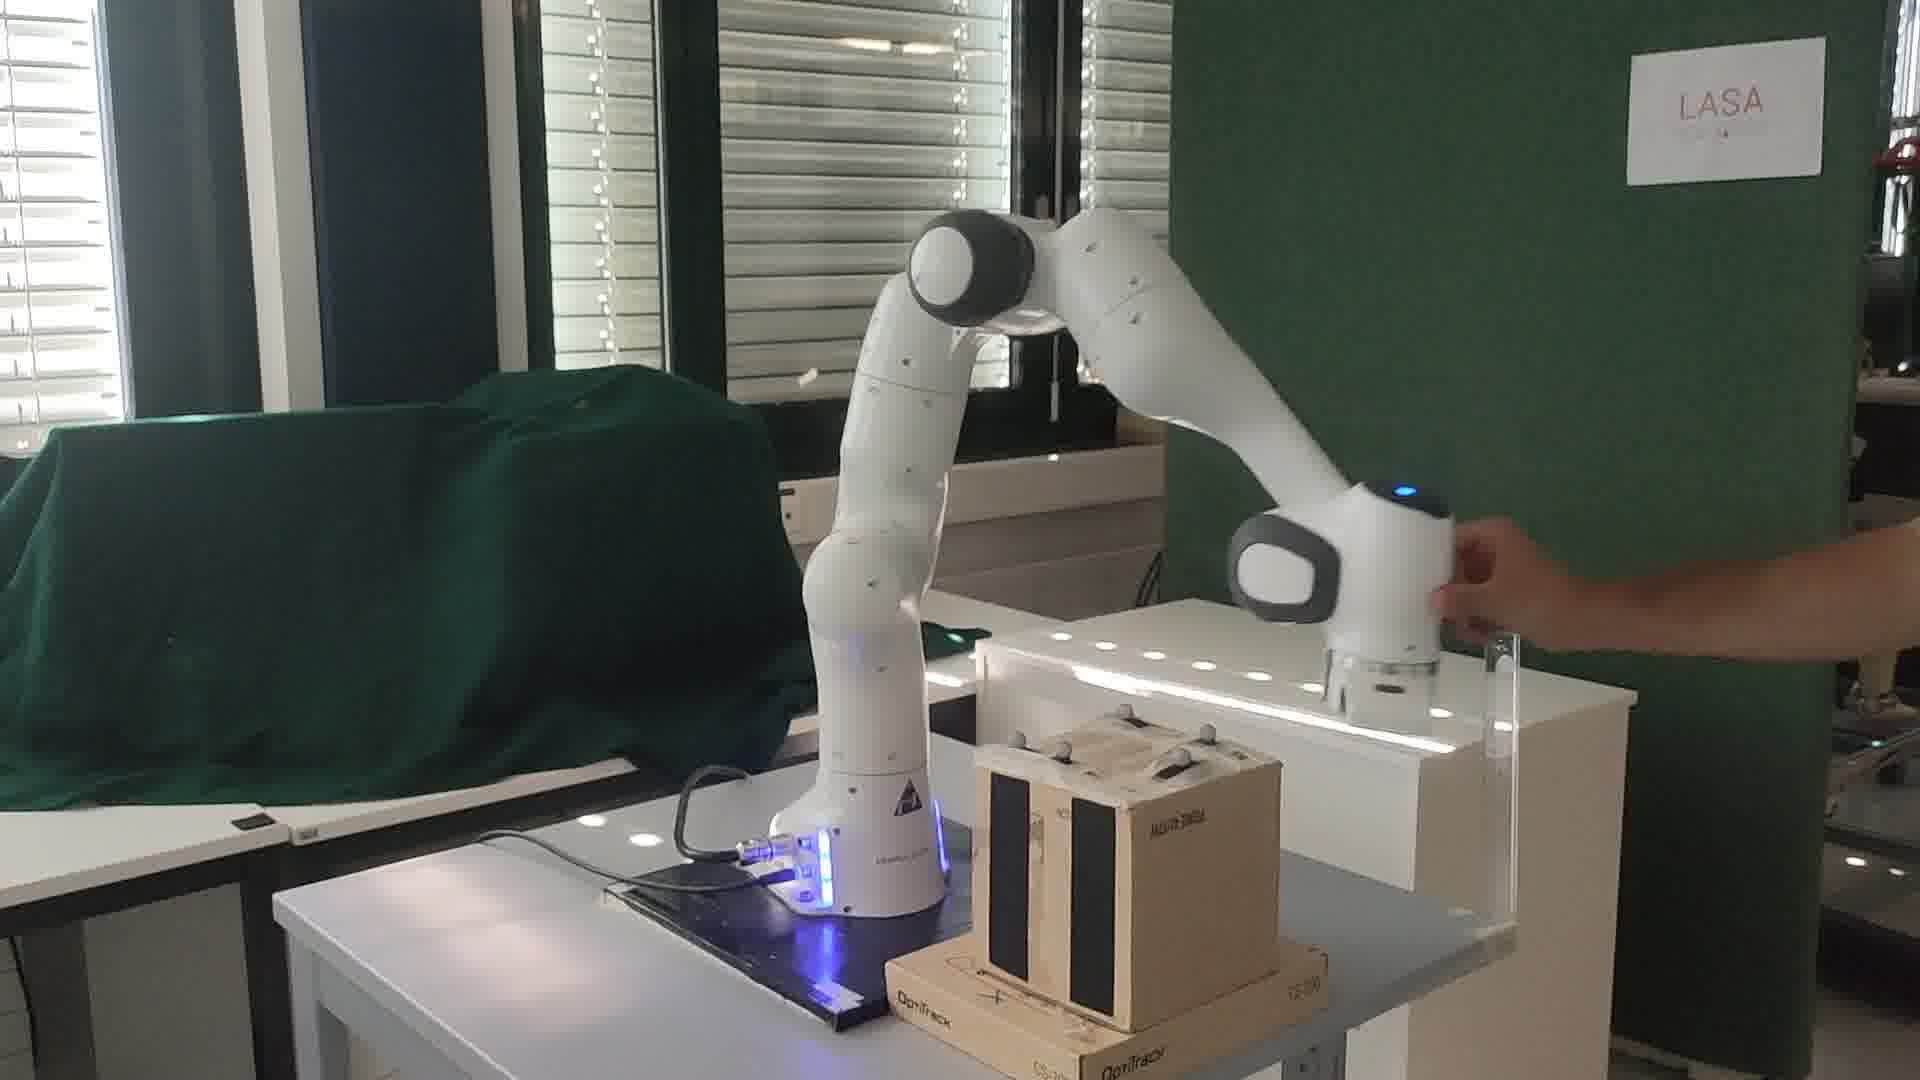
\includegraphics[width=-1.33\textwidth]{figures/franka_sequence/franka_velocity_conserving023}\hfill%
    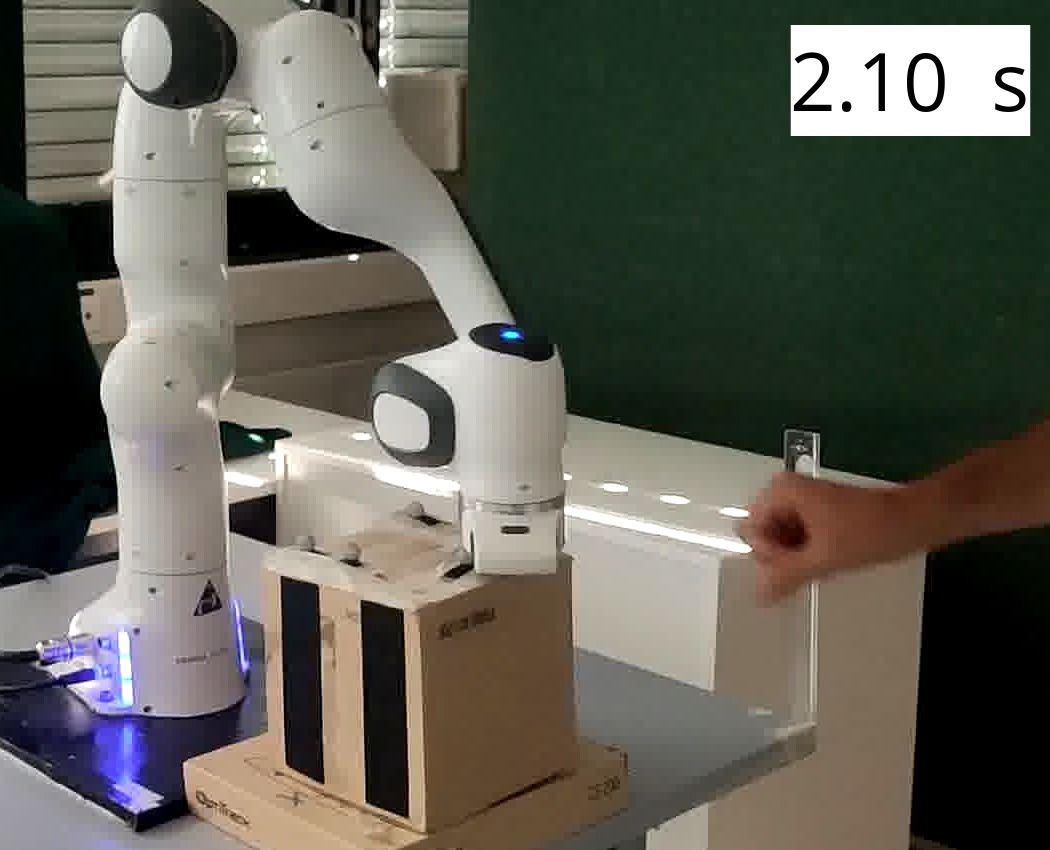
\includegraphics[width=0.4\textwidth]{figures/franka_sequence/franka_velocity_conserving025}\hfill%
      \caption{Velocity preserving controller leads to collision with obstacle}
      \label{fig:franka_sequence_obstacle_aware}
    \end{subfigure}
	\caption{The robot arm, guided by the obstacle-aware passive controller, effectively avoids the disturbance towards the obstacle while maintaining a margin of \qty{0.16}{m} around the obstacle.}
	\label{fig:instances_evaluation_on_robot_arm}
\end{figure}

\begin{figure}[htbp]
    \begin{subfigure}{\columnwidth}
      \centerline{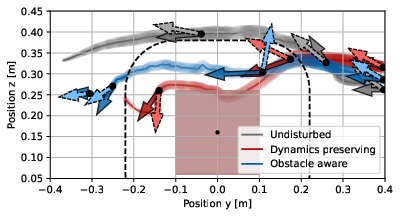
\includegraphics[width=\textwidth]{figures/robot_arm_trajectory_xyz}}
      \caption{The two control methods compared with the undisturbed trajectory. The wider line indicates a higher x-value. The darker arrow is the actual, and the desired velocity is brighter arrow.}
      \label{fig:robot_arm_trajectory_xyz}
    \end{subfigure}
    \begin{subfigure}{\columnwidth}
		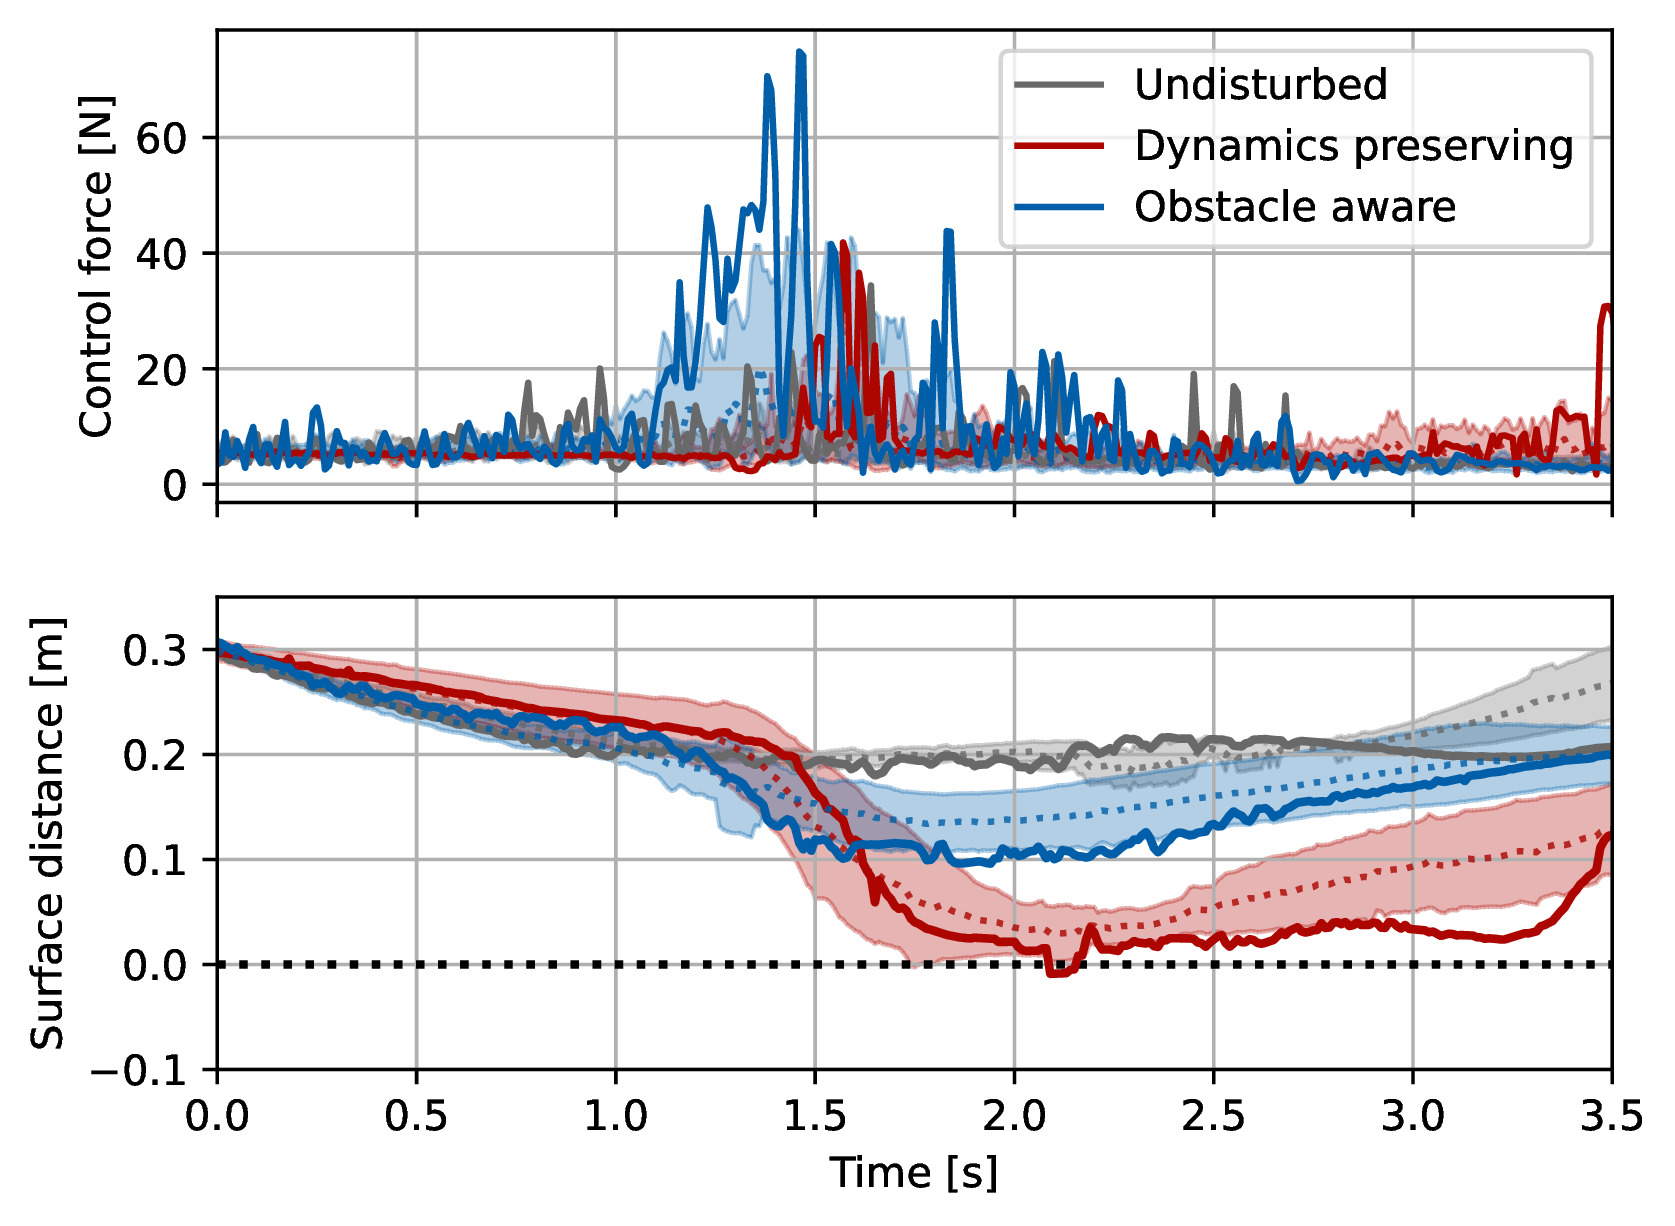
\includegraphics[width=\textwidth]{figures/trajectory_comparison_force_and_distance}
      \caption{The specific trajectory is represented by a full line, while the average (dashed line) and variance (shaded area) are evaluated over ten epochs. The control force's mean and variance are evaluated in the logarithmic space.}
      \label{fig:trajectory_comparison_force_and_distance}
    \end{subfigure}
	\caption{
 The experiment was repeated ten times with a similar disturbance applied to the robot arm in each run.
 }  
    \label{fig:evaluation_on_robot_arm}
\end{figure}
\
\else
\begin{figure}
    \centering
   \begin{subfigure}{\columnwidth}
    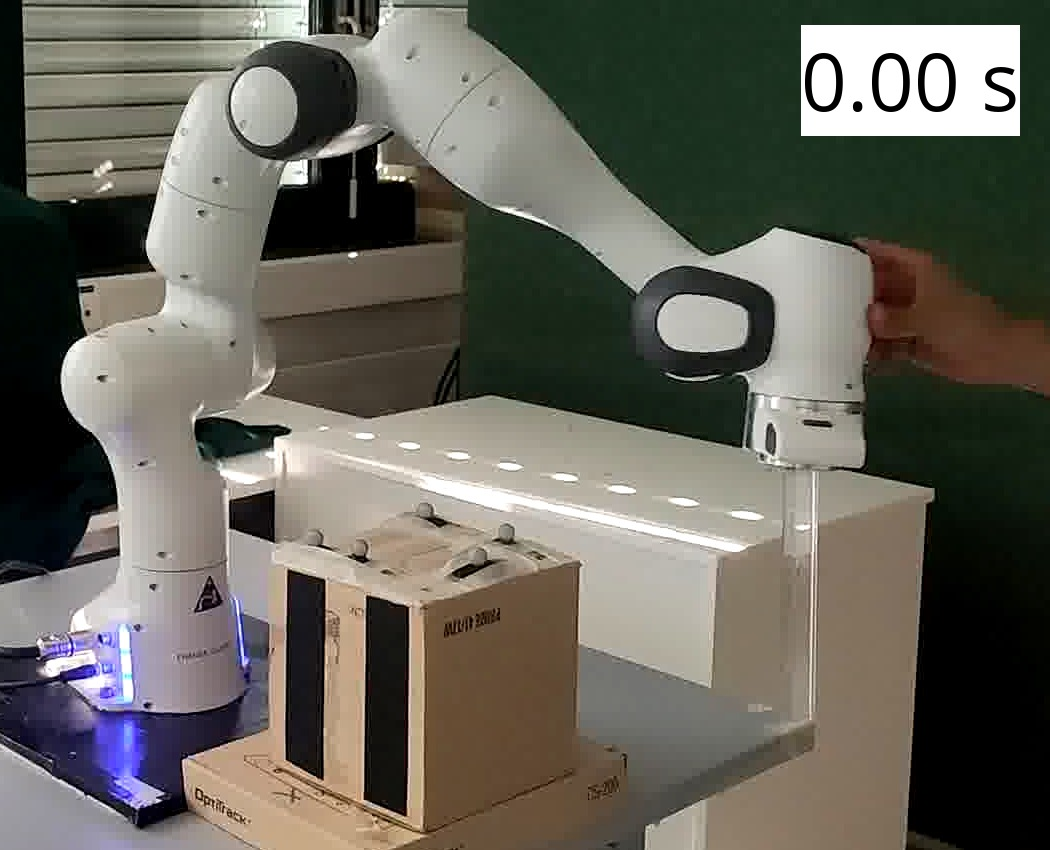
\includegraphics[width=0.49\textwidth]{figures/franka_sequence/franka_obstacle_aware016}\hfill%
    % 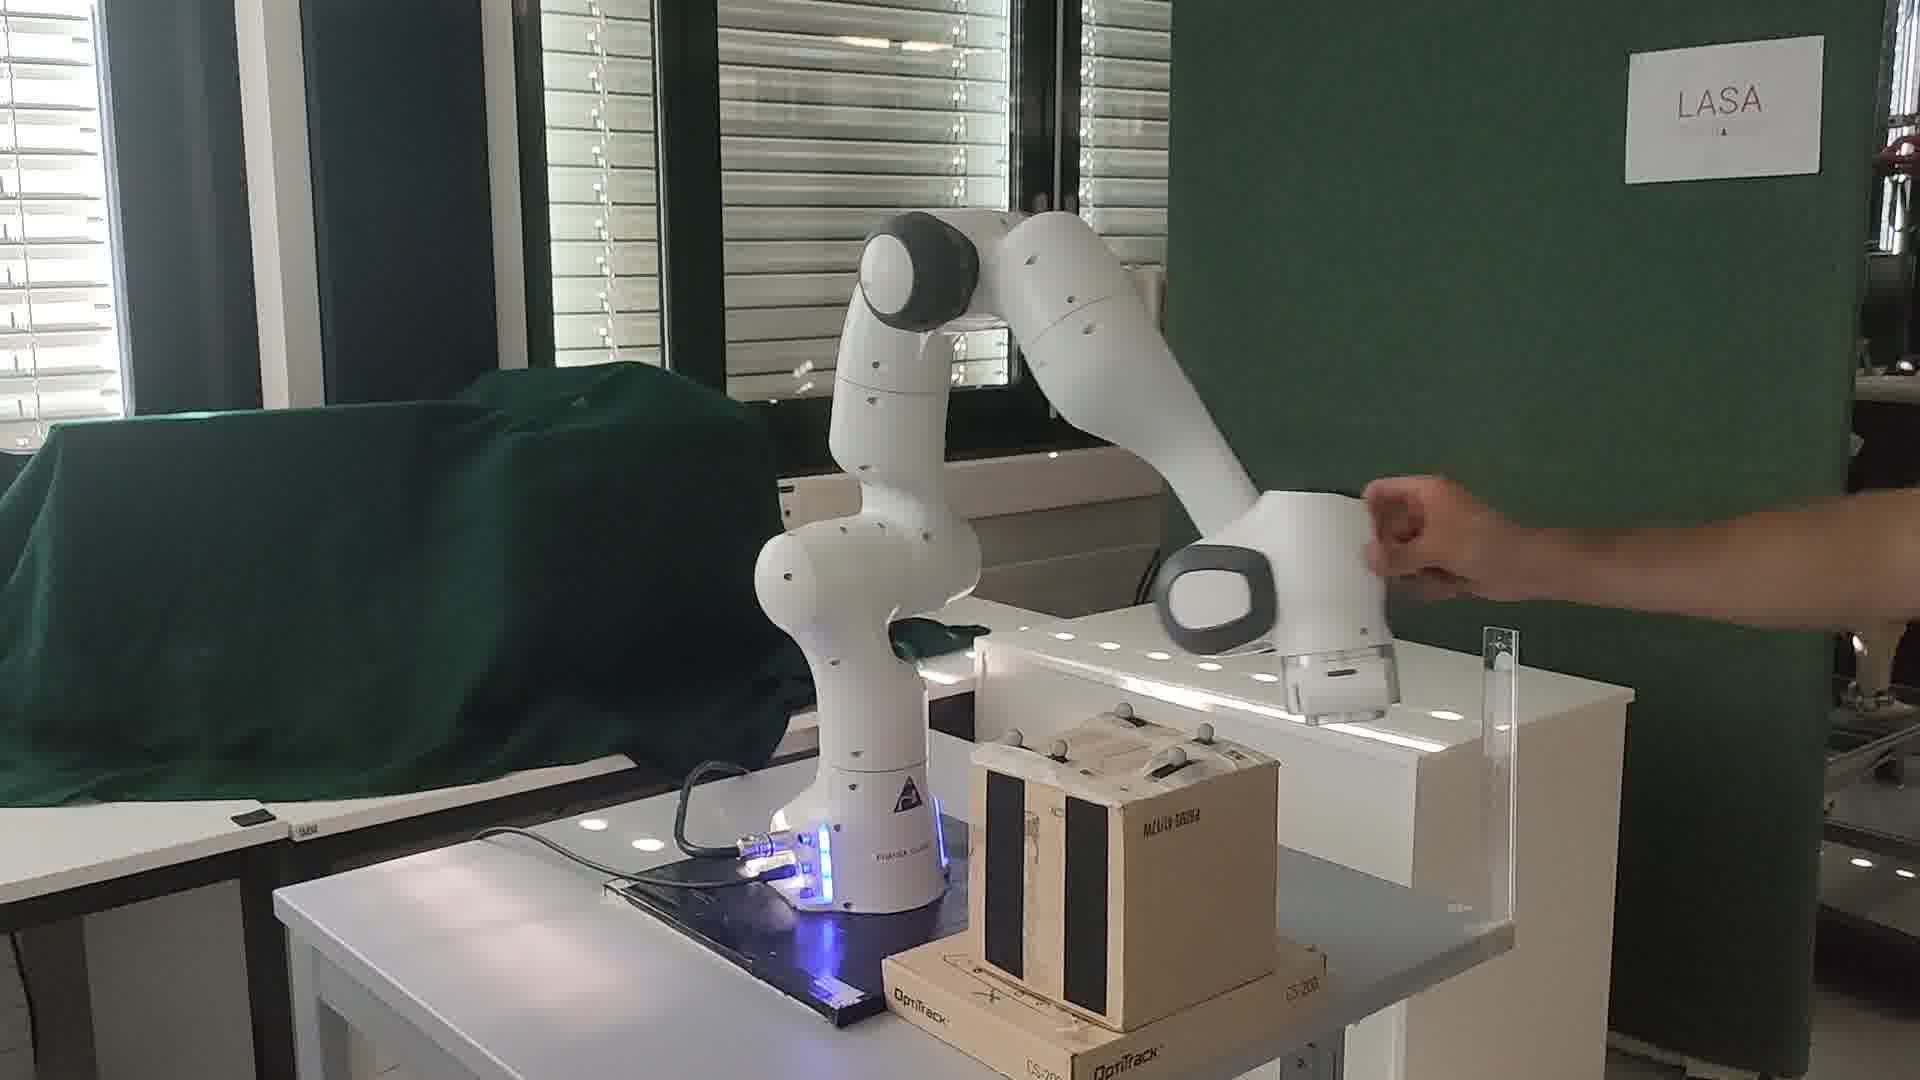
\includegraphics[width=0.33\textwidth]{figures/franka_sequence/franka_obstacle_aware018}\hfill%
    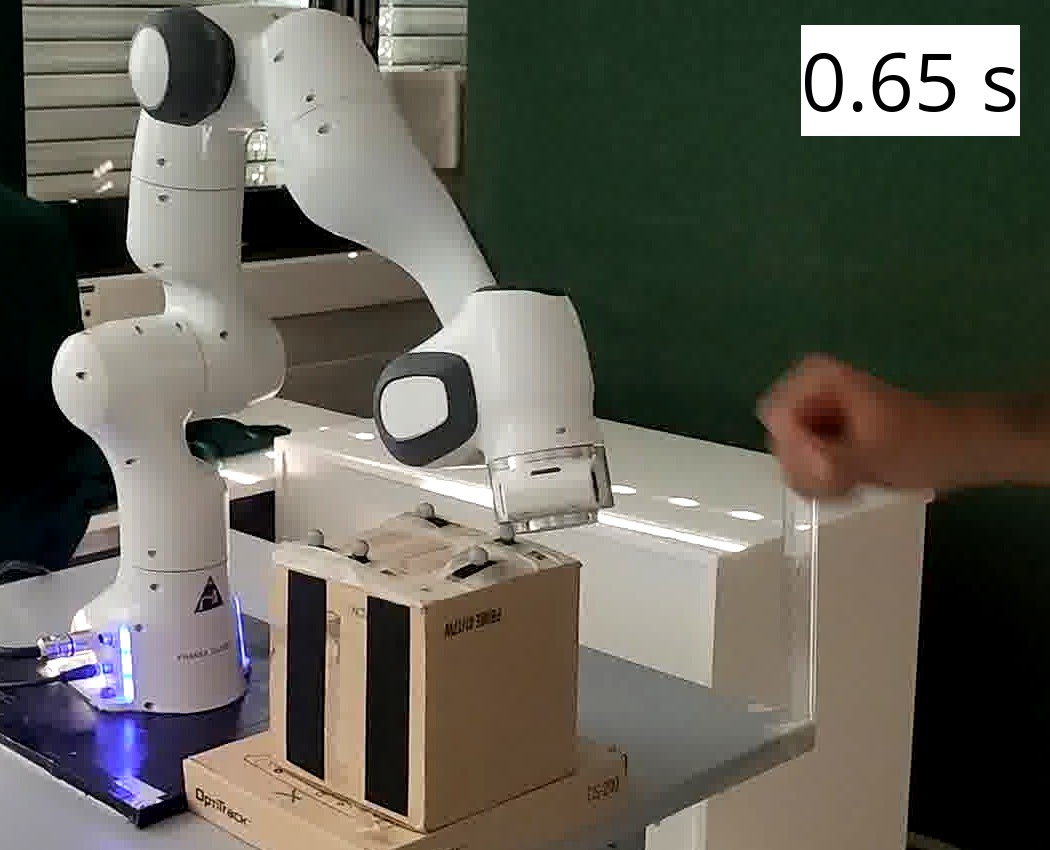
\includegraphics[width=0.49\textwidth]{figures/franka_sequence/franka_obstacle_aware020}
      \caption{Obstacle-aware controller rejects repulsion and avoids collision}
      \label{fig:franka_sequence_obstacle_aware}
    \end{subfigure}
	\begin{subfigure}{\columnwidth}
    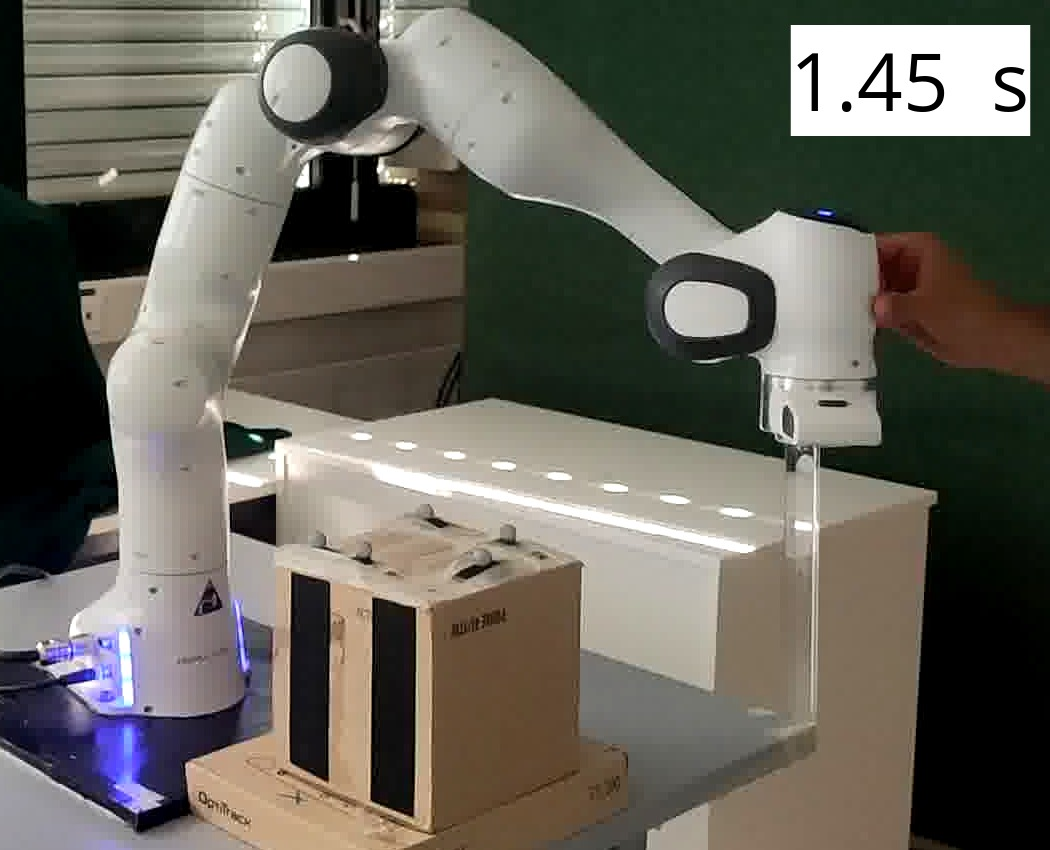
\includegraphics[width=0.49\textwidth]{figures/franka_sequence/franka_velocity_conserving021}\hfill%
    % 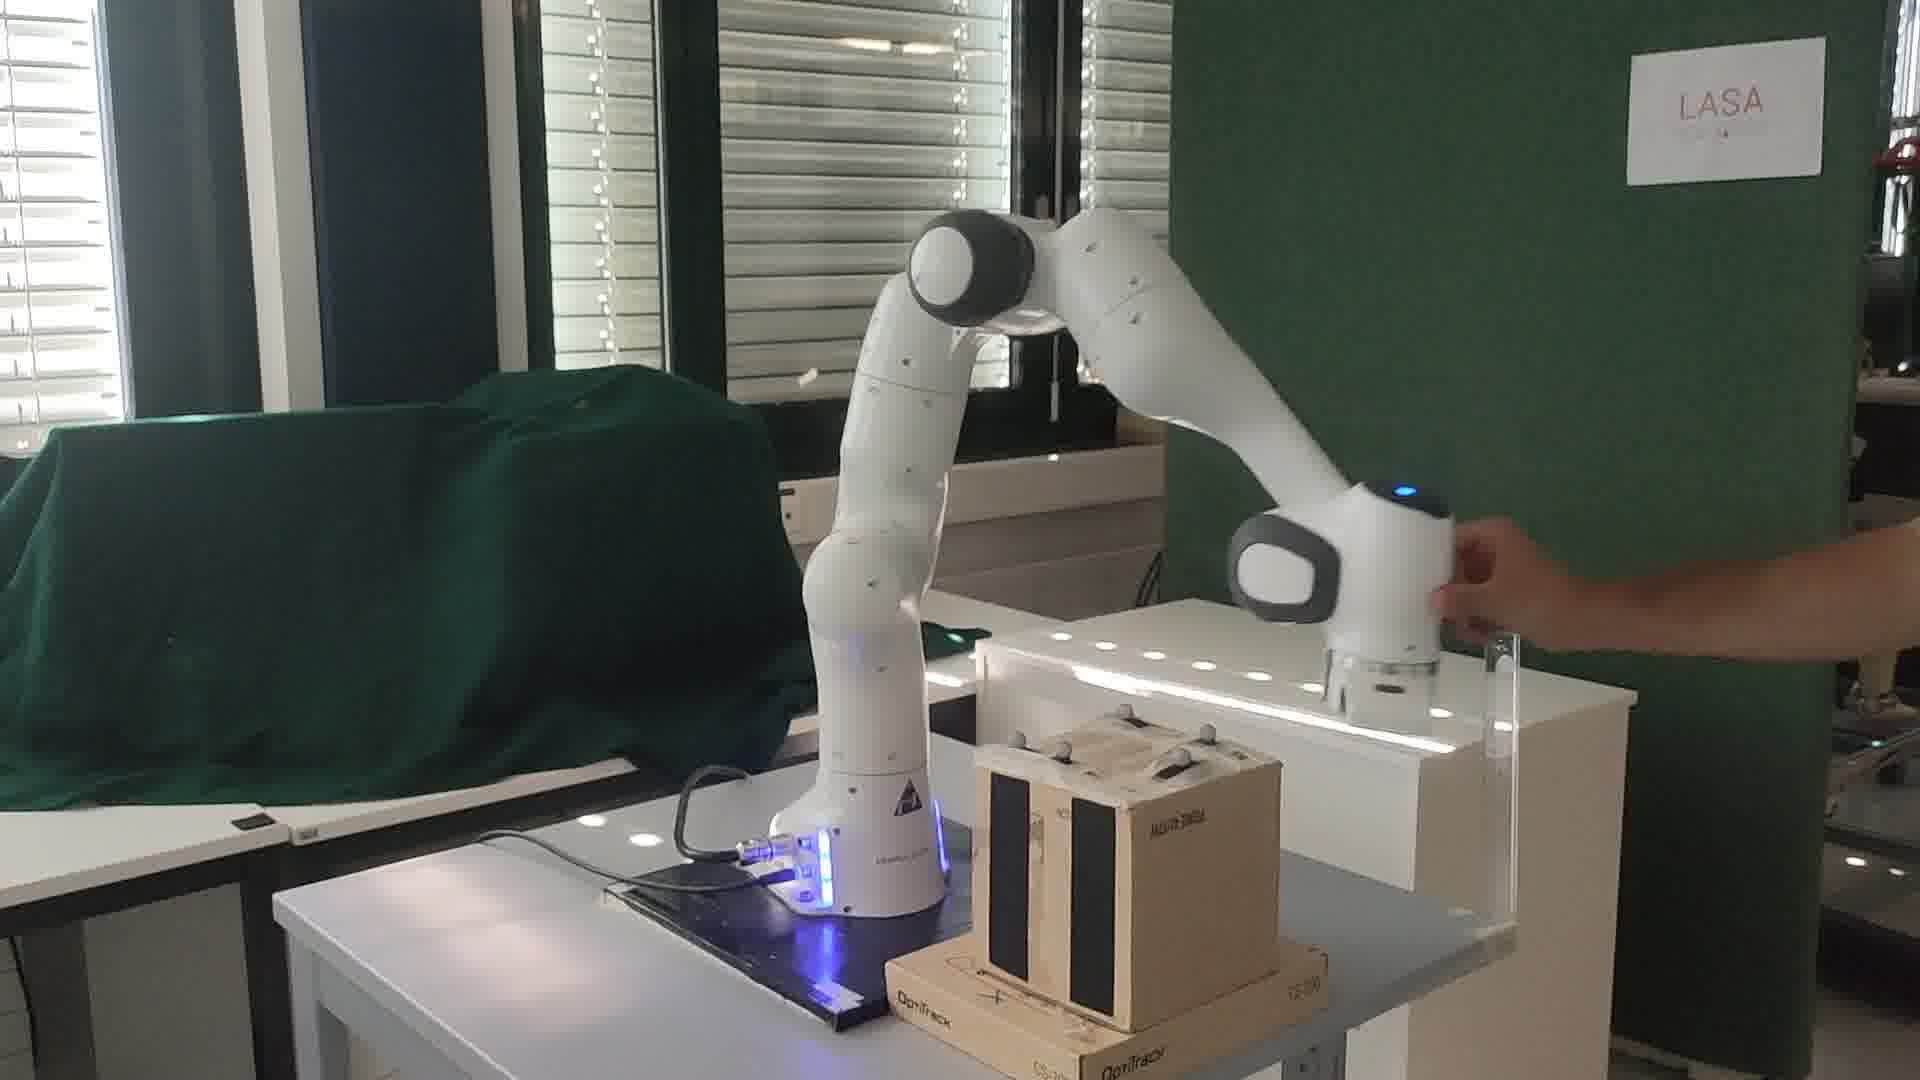
\includegraphics[width=-1.33\textwidth]{figures/franka_sequence/franka_velocity_conserving023}\hfill%
    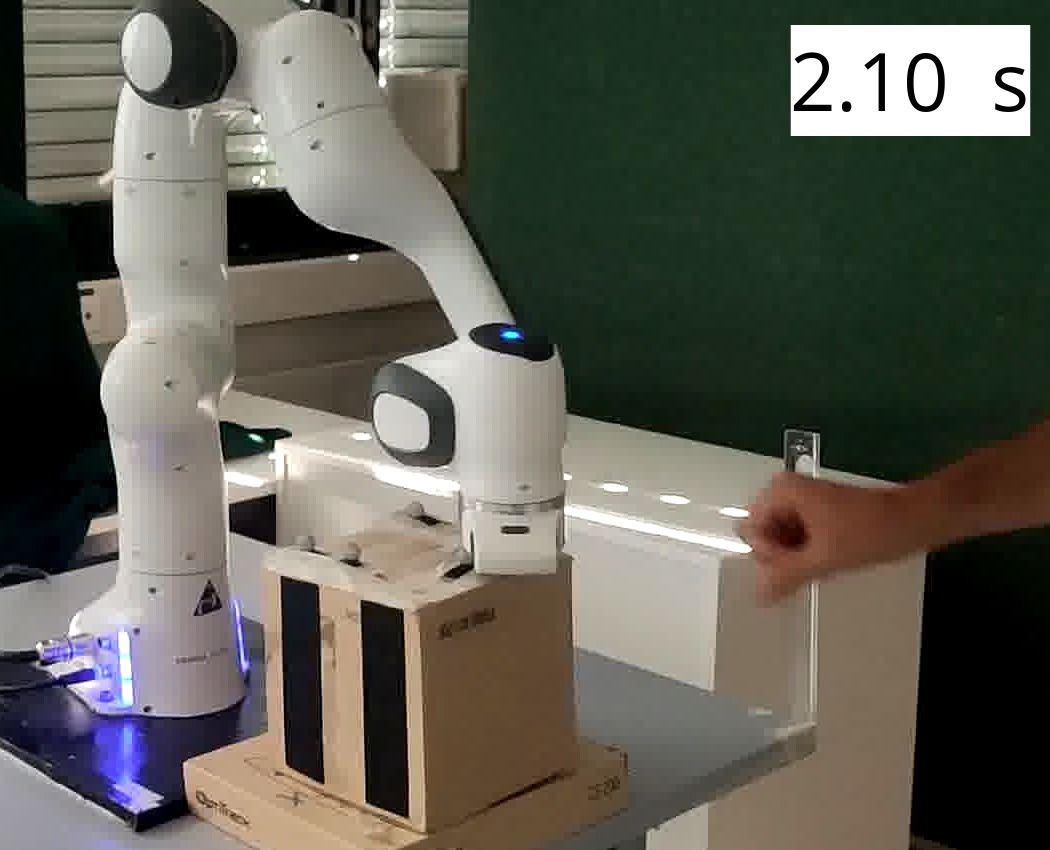
\includegraphics[width=0.49\textwidth]{figures/franka_sequence/franka_velocity_conserving025}\hfill%
      \caption{Velocity preserving controller leads to collision with obstacle}
      \label{fig:franka_sequence_obstacle_aware}
    \end{subfigure}
%    \caption{Comparison of the two control methods}
%    \label{fig:evaluation_on_robot_arm}
% \end{figure}
% \begin{figure}
%     \centering
    \begin{subfigure}{\columnwidth}
      \centerline{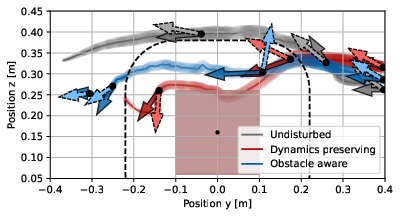
\includegraphics[width=\textwidth]{figures/robot_arm_trajectory_xyz}}
      \caption{The two control methods compared with the undisturbed trajectory. The wider line indicates a higher x-value. The darker arrow is the actual, and the desired velocity is brighter arrow.}
      \label{fig:robot_arm_trajectory_xyz}
    \end{subfigure}
    \begin{subfigure}{\columnwidth}
		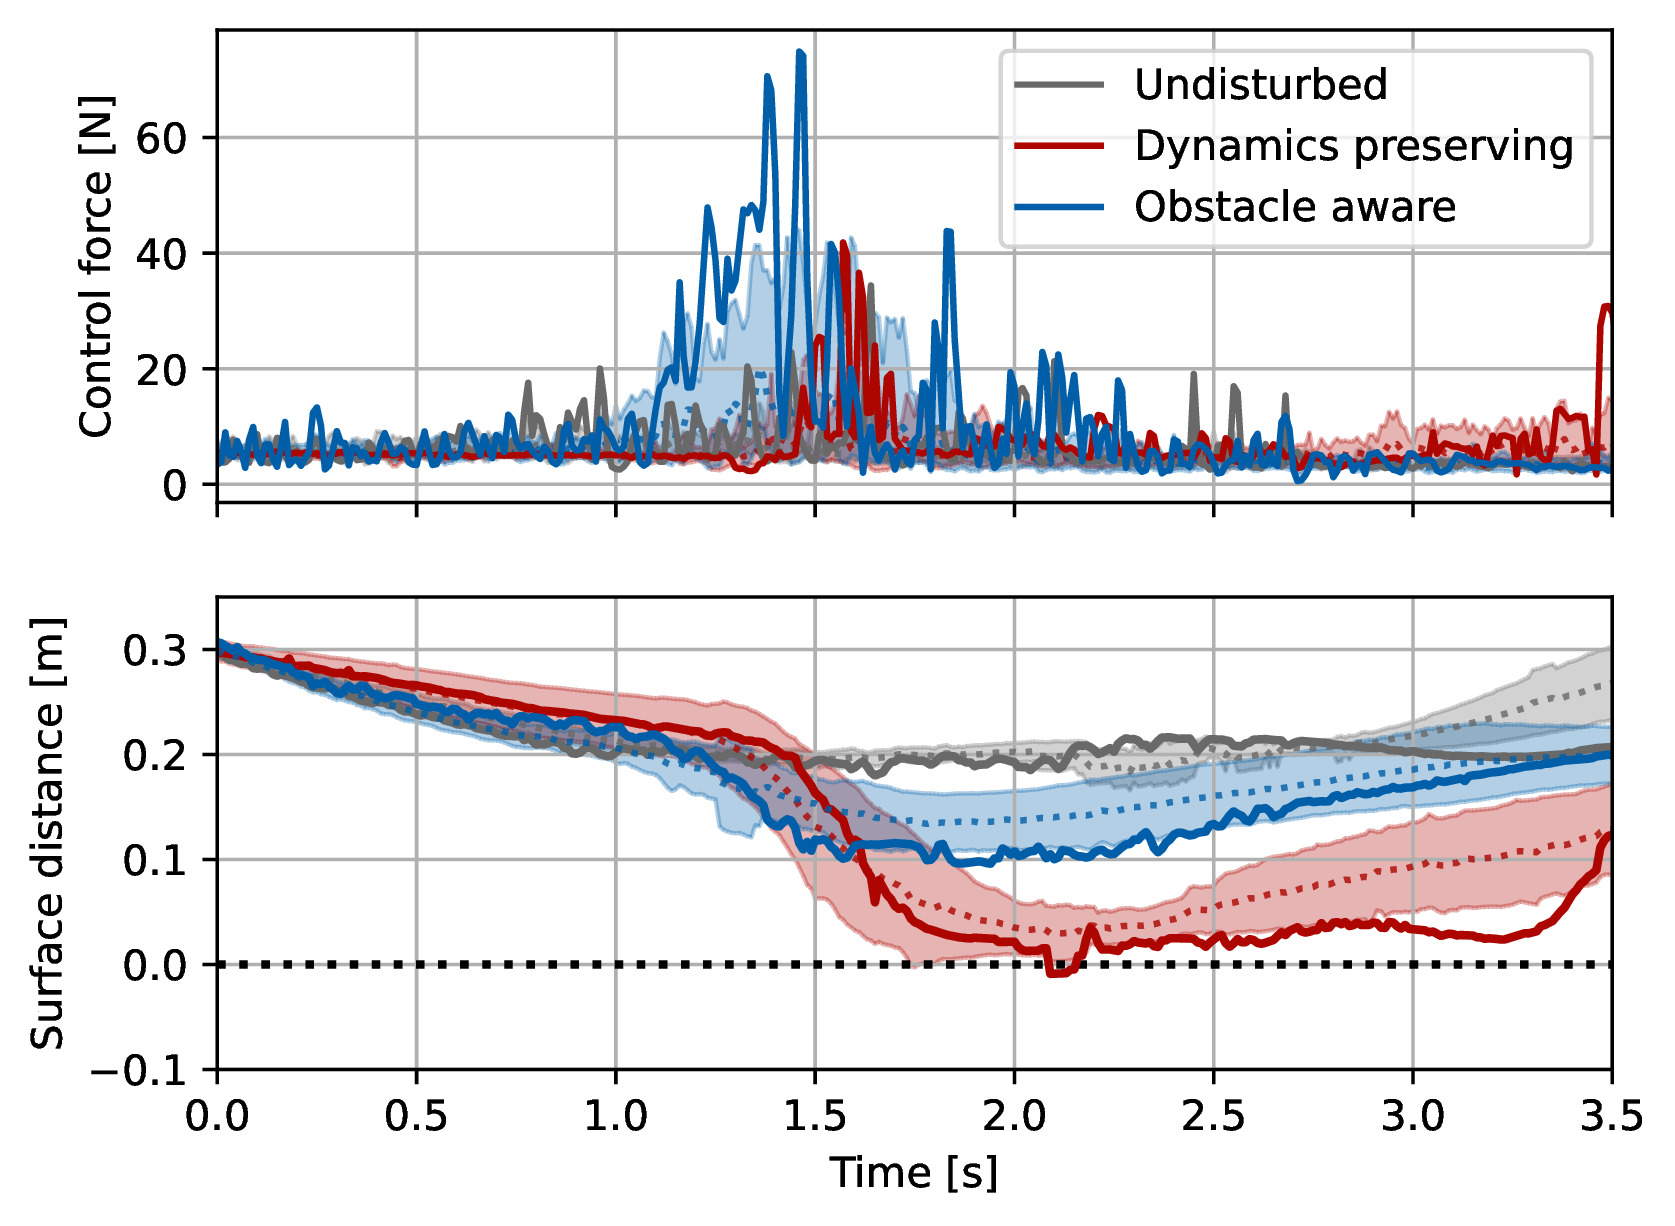
\includegraphics[width=\textwidth]{figures/trajectory_comparison_force_and_distance}
      \caption{The specific trajectory is represented by a full line, while the average (dashed line) and variance (shaded area) are evaluated over ten epochs. The control force's mean and variance are evaluated in the logarithmic space.}
      \label{fig:trajectory_comparison_force_and_distance}
    \end{subfigure}
	\caption{
The robot arm, guided by the obstacle-aware passive controller, effectively avoids the disturbance towards the obstacle while maintaining a margin of \qty{0.16}{m} around the obstacle. The experiment was repeated ten times with a similar disturbance applied to the robot arm in each run.
 }  
    \label{fig:evaluation_on_robot_arm}
\end{figure}
\fi

\section{Discussion}
We introduced a novel passive obstacle-aware controller that takes as an input the desired, collision-free velocity and outputs a control torque. 
The stability proof enables the controller to be used with any bounded input velocity field, and this result extends to a general class of damping controllers.
Furthermore, the controller is shown to reject disturbances, and the parameter-tuning for the discrete-time system has been analyzed. 

The controller was experimentally evaluated and compared to a baseline passive controller. The proposed approach shows increased resistance to noise, both in position and velocity and improved tracking. Finally, disturbance force on a real robot arm could be successfully rejected to ensure collision avoidance while following a simple trajectory.

\subsection{Discrete Control Convergence}
The proposed controller is only stable but does not ensure convergence. However, convergence could be achieved by modifying the controller by introducing an additional proportional term, as is common in impedance controllers:
\begin{equation}
	\vecs{\tau_c} = \vect g (\vecs\xi) 
	% + \matd{D}(\vect \xi, \dot{\vect \xi}) \dot{\vect \xi}  
	+ \matd{D}(\vecs\xi) \left(\vecs f(\vecs\xi) - \vecs{\dot\xi} \right) 
	+ \matd{K}(\vecs \xi) \left(\vecs \xi - \vecs \xi^a \right)
\label{eq:control_command_proportional}
\end{equation}
However, this design interferes with the basis passive controller, and the convergence towards the attractor is facilitated by (stable) velocity $\vect f(\vecs \xi)$. 
Moreover, introducing a variable damping matrix will result in a potentially unstable system, as the passivity proof no longer holds.
Future work should further analyze how to include dynamics properties in the design of the damping parameters for improved system performance.

\subsection{Applicability and Theoretical Analysis}
The theoretical analysis from Theorem~\ref{theorem:passivity} indicates BIBO stability for a system with bounded desired velocity. Consequently, controllers like the damping-based approach in \parencite{kronander2015passive} do not require an energy tank. Yet, introducing an adaptive proportional term $\mathcal{K}$ can lead to instabilities \parencite{ferraguti2013tank, kronander2016stability}. 
Careful consideration of the controller design and stability analysis is necessary to ensure robust and safe performance in practical applications. 
Nevertheless, the passivity proof enables a broad range of time-varying damping controllers to be safely applied to robotic systems.

\subsection{Point Mass Agents}
While the controller is limited to a point mass representation of the robot, its computational efficiency would allow multiple evaluations along the robot arm. This could be used to ensure full body control of the robot, hence improving the system's safety.

\subsection{Caution in Obstacle's Proximity}
In this work, we assume the obstacles' position to be precisely known. However, in many scenarios, the robot might have limited perception as it approaches an obstacle. Hence, the robot should be more compliant to enable safe workspace exploration rather than increasing the damping. Future work should explore how to combine these two opposing paradigms: safe control for avoidance, yet cautious exploration.
